%
% Chapter 7: Optimizers and Learning Rate Schedulers

\clearpage
\cleardoublepage

\chapter{Optimizers and Learning Rate Schedulers}

\section{Gradient Descent Optimization}

Training neural networks minimizes a loss function by updating parameters in the direction that reduces loss.

\subsection{Batch Gradient Descent}

Updates parameters using the gradient of the entire dataset:
\begin{equation}
\theta_{t+1} = \theta_t - \alpha \nabla_\theta \mathcal{L}(\theta_t)
\end{equation}

\begin{itemize}
    \item \textbf{Advantages:} Stable convergence, exact gradient
    \item \textbf{Disadvantages:} Slow for large datasets, memory intensive
\end{itemize}

\subsection{Stochastic Gradient Descent (SGD)}

Updates parameters using gradient of a single sample:
\begin{equation}
\theta_{t+1} = \theta_t - \alpha \nabla_\theta \mathcal{L}(\theta_t; \mathbf{x}^{(i_t)}, \mathbf{y}^{(i_t)})
\end{equation}

\begin{itemize}
    \item \textbf{Advantages:} Fast, escapes local minima, online learning
    \item \textbf{Disadvantages:} Noisy gradients, requires smaller learning rate
\end{itemize}

\subsection{Mini-Batch Gradient Descent}

Updates using a batch of $B$ samples:
\begin{equation}
\theta_{t+1} = \theta_t - \alpha \frac{1}{B}\sum_{i=1}^{B}\nabla_\theta \mathcal{L}(\theta_t; \mathbf{x}^{(i)}, \mathbf{y}^{(i)})
\end{equation}

This is the standard approach in deep learning.

\section{Gradient Descent with Momentum}

Momentum accelerates convergence by accumulating velocity:
\begin{align}
\mathbf{v}_{t+1} &= \beta \mathbf{v}_t + (1-\beta)\nabla_\theta \mathcal{L}(\theta_t) \\
\theta_{t+1} &= \theta_t - \alpha \mathbf{v}_{t+1}
\end{align}

\begin{itemize}
    \item $\beta \in [0, 1)$ is the momentum coefficient (typically 0.9)
    \item \textbf{Reduces oscillations} in steep directions
    \item \textbf{Accelerates convergence} in shallow directions
\end{itemize}

\begin{note}[Nesterov Accelerated Gradient]
Nesterov momentum looks ahead:
\begin{align}
\mathbf{v}_{t+1} &= \beta \mathbf{v}_t - \alpha \nabla_\theta \mathcal{L}(\theta_t + \beta\mathbf{v}_t) \\
\theta_{t+1} &= \theta_t + \mathbf{v}_{t+1}
\end{align}
This provides better convergence guarantees and often faster training.
\end{note}

\section{Adaptive Learning Rate Methods}

These methods adjust learning rates per-parameter based on gradient history.

\subsection{AdaGrad}

Adapts learning rate inversely proportional to accumulated squared gradients:
\begin{align}
\mathbf{g}_t &= \nabla_\theta \mathcal{L}(\theta_t) \\
\mathbf{r}_t &= \mathbf{r}_{t-1} + \mathbf{g}_t \odot \mathbf{g}_t \\
\theta_{t+1} &= \theta_t - \frac{\alpha}{\sqrt{\mathbf{r}_t + \epsilon}} \odot \mathbf{g}_t
\end{align}

\begin{itemize}
    \item \textbf{Good for sparse features}
    \item \textbf{Learning rate decreases} over time
    \item \textbf{May stop too early} in deep learning
\end{itemize}

\subsection{RMSProp}

Exponentially weighted moving average of squared gradients:
\begin{align}
\mathbf{g}_t &= \nabla_\theta \mathcal{L}(\theta_t) \\
\mathbf{r}_t &= \beta \mathbf{r}_{t-1} + (1-\beta)\mathbf{g}_t \odot \mathbf{g}_t \\
\theta_{t+1} &= \theta_t - \frac{\alpha}{\sqrt{\mathbf{r}_t + \epsilon}} \odot \mathbf{g}_t
\end{align}

\begin{itemize}
    \item \textbf{Addresses AdaGrad's diminishing learning rate}
    \item \textbf{Common default for RNNs}
    \item $\beta = 0.9$ is typical
\end{itemize}

\subsection{Adam (Adaptive Moment Estimation)}

Combines momentum and RMSProp:
\begin{align}
\mathbf{m}_t &= \beta_1 \mathbf{m}_{t-1} + (1-\beta_1)\mathbf{g}_t \quad \text{(first moment)} \\
\mathbf{v}_t &= \beta_2 \mathbf{v}_{t-1} + (1-\beta_2)\mathbf{g}_t^2 \quad \text{(second moment)} \\
\hat{\mathbf{m}}_t &= \frac{\mathbf{m}_t}{1-\beta_1^t} \quad \text{(bias correction)} \\
\hat{\mathbf{v}}_t &= \frac{\mathbf{v}_t}{1-\beta_2^t} \\
\theta_{t+1} &= \theta_t - \frac{\alpha \hat{\mathbf{m}}_t}{\sqrt{\hat{\mathbf{v}}_t} + \epsilon}
\end{align}

\begin{properties}[Adam Properties]
\begin{itemize}
    \item \textbf{Default optimizer} for most deep learning tasks
    \item \textbf{Robust to hyperparameters}
    \item \textbf{Default parameters:} $\alpha = 0.001, \beta_1 = 0.9, \beta_2 = 0.999, \epsilon = 10^{-8}$
    \item \textbf{Bias correction} for early time steps
\end{itemize}
\end{properties}

\begin{code}
    \captionof{listing}{Optimizers in PyTorch}
    \label{code:optimizers}
\begin{lstlisting}[language=python]
import torch.optim as optim

# SGD with momentum
optimizer = optim.SGD(model.parameters(), lr=0.01, momentum=0.9)

# SGD with Nesterov momentum
optimizer = optim.SGD(model.parameters(), lr=0.01, momentum=0.9, nesterov=True)

# Adam
optimizer = optim.Adam(model.parameters(), lr=0.001, betas=(0.9, 0.999))

# AdamW (decoupled weight decay)
optimizer = optim.AdamW(model.parameters(), lr=0.001, weight_decay=0.01)

# RMSProp
optimizer = optim.RMSprop(model.parameters(), lr=0.01, alpha=0.99)
\end{lstlisting}
\end{code}

\subsection{AdamW (Adam with Weight Decay)}

Decouples weight decay from gradient update:
\begin{equation}
\theta_{t+1} = \theta_t - \alpha \frac{\mathbf{m}_t}{\sqrt{\mathbf{v}_t} + \epsilon} - \alpha \lambda \theta_t
\end{equation}

\begin{itemize}
    \item \textbf{Proper L2 regularization} unlike original Adam
    \item \textbf{Better generalization} in many tasks
    \item \textbf{Standard in transformers}
\end{itemize}

\section{Gradient Clipping}

Prevents exploding gradients:
\begin{equation}
\mathbf{g} = \text{clip}(\nabla_\theta \mathcal{L}, -\text{clip\_value}, \text{clip\_value})
\end{equation}

Common values: clip\_value = 1.0 to 5.0

Essential for RNNs and Transformers.

\section{Learning Rate Schedulers}

Learning rate schedules adjust the learning rate during training.

\subsection{Step Decay}

\begin{equation}
\alpha_t = \alpha_0 \cdot \gamma^{\lfloor t / T \rfloor}
\end{equation}
where $\gamma$ is the decay factor (e.g., 0.5) and $T$ is the period.

\subsection{Exponential Decay}

\begin{equation}
\alpha_t = \alpha_0 \cdot e^{-\lambda t}
\end{equation}

\subsection{Cosine Annealing}

\begin{equation}
\alpha_t = \alpha_{min} + \frac{1}{2}(\alpha_{max} - \alpha_{min})\left(1 + \cos\left(\frac{t\pi}{T}\right)\right)
\end{equation}

\begin{figure}[h]
    \centering
    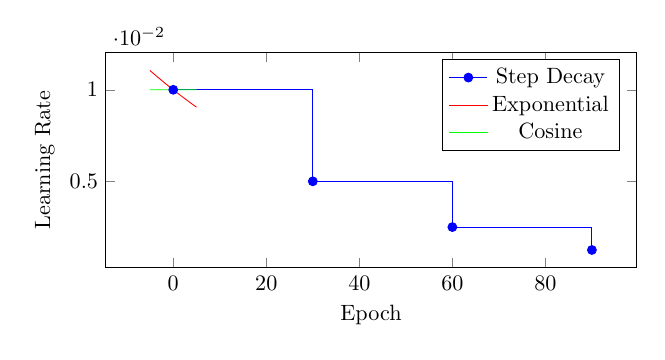
\begin{tikzpicture}[scale=0.8]
        \begin{axis}[
            xlabel=Epoch,
            ylabel=Learning Rate,
            width=10cm,
            height=5cm,
            legend pos=north east
        ]
            % Step decay
            \addplot[blue, const plot, mark=*] coordinates {
                (0, 0.01)
                (30, 0.005)
                (60, 0.0025)
                (90, 0.00125)
            };
            \addlegendentry{Step Decay}
            
            % Exponential
            \addplot[red, smooth] {0.01 * exp(-0.02*x)};
            \addlegendentry{Exponential}
            
            % Cosine
            \addplot[green, smooth] {(0.001 + 0.5*(0.01-0.001)*(1+cos(pi*x/100))};
            \addlegendentry{Cosine}
        \end{axis}
    \end{tikzpicture}
    \caption{Learning rate schedules}
    \label{fig:lr_schedules}
\end{figure}

\subsection{Warmup}

Gradually increase learning rate at the start:
\begin{equation}
\alpha_t = \alpha_{max} \cdot \frac{t}{T_{warmup}} \quad \text{for } t < T_{warmup}
\end{equation}

\begin{itemize}
    \item \textbf{Prevents large gradients} at the start
    \item \textbf{Important for transformers}
    \item \textbf{Common: 500-10000 warmup steps}
\end{itemize}

\section{Optimizer Selection}

\begin{table}[h]
    \centering
    \caption{Optimizer Selection Guide}
    \begin{tabular}{L{2.5cm} L{3cm} L{3.5cm}}
        \toprule
        \textbf{Optimizer} & \textbf{Good for} & \textbf{Notes} \\
        \midrule
        SGD + Momentum & Image classification & Best generalization \\
        Adam & General purpose & Default choice \\
        AdamW & Transformers, NLP & Best for fine-tuning \\
        RMSProp & RNNs & Good for recurrent models \\
        \bottomrule
    \end{tabular}
\end{table}

\section{Chapter Summary}

\begin{enumerate}
    \item Gradient descent is the foundation of neural network optimization
    \item Momentum accelerates convergence by accumulating velocity
    \item Adam combines momentum and adaptive learning rates
    \item AdamW provides proper weight decay regularization
    \item Learning rate schedulers improve convergence
    \item Warmup is important for transformer training
\end{enumerate}
